\documentclass{article}

% ─────────────────────────── PACKAGES ────────────────────────────
\usepackage{times}
\usepackage{geometry}
\geometry{a4paper,left=0.6cm,right=0.7cm,top=1cm,bottom=1cm,columnsep=0.8cm}

\usepackage{fontawesome}
\usepackage[hidelinks]{hyperref}
\usepackage{paracol}
\usepackage{tikz}
\usepackage{tabularx}
\usepackage{ragged2e}
\usepackage{xcolor}
\usepackage{enumitem}


\definecolor{maincolor}{HTML}{ffffff}
\definecolor{seccolor}{HTML}{0b1f3b}
\definecolor{gray}{HTML}{8c94a9}
\definecolor{sidetext}{HTML}{59cee5}
\definecolor{Green}{HTML}{2caf00}
\definecolor{lightgray}{HTML}{D3D3D3}
%\definecolor{maincolor}{HTML}{2AAEE7}

\newcolumntype{Y}{>{\RaggedRight\arraybackslash}X}
\setlist[itemize]{itemsep=-2pt,topsep=0pt,leftmargin=*}
\renewcommand{\labelitemi}{\textcolor{black}{\footnotesize$\bullet$}}
%
\setlength{\parindent}{0pt}

% titre de section
\newcommand{\cvsection}[1]{%
  \par\bigskip
  \begin{tabular}{@{}p{\linewidth}}
  \textbf{\Large #1}\\[3pt]\hline
  \end{tabular}\medskip}

\newcommand*{\ClipSep}{0.4cm}

\setlength{\columnseprule}{0.4pt}        % épaisseur du trait
\setlength{\columnsep}{0.8cm}            % (facultatif : rappel de l’écart)
\def\columnseprulecolor{\color{lightgray}}% couleur du trait
% ─────────────────────────── DOCUMENT ────────────────────────────
\begin{document}\pagestyle{empty}
\columnratio{0.7}\begin{paracol}{2}

%%%%%%%%%%%%%%%%%%%%%%%%%%%%%%%%%%%%%%%%%%%%%%%%%%%%%%%%%%%%%%%%%%%
% Colonne gauche (70 %)
%%%%%%%%%%%%%%%%%%%%%%%%%%%%%%%%%%%%%%%%%%%%%%%%%%%%%%%%%%%%%%%%%%%

{\LARGE\textbf{Judikael MOUROUVIN}}

\bigskip
{\color{sidetext}\Large\textbf{Technicien informatique \& marketing digital}}

\medskip
\begin{tabular}{@{}cp{0.4\linewidth}cp{0.4\linewidth}}
  \color{sidetext}\faEnvelope & \href{mailto:jkmou971@gmail.com}{jkmou971@gmail.com} &
  \color{sidetext}\faMapMarker & Route de COCOYER\;97190 GOSIER\\[6pt]
  \color{sidetext}\faPhone & \href{tel:+590 0690 91 14 48}{+590 0690 91 14 48} &
  \color{sidetext}\faLinkedin & \href{}{}
\end{tabular}

\cvsection{EXPERIENCE}

\colorbox{maincolor}{%
  \begin{minipage}{\linewidth}
    \textbf{Alternant en marketing digital} \\ Mairie du Gosier – DSI \\ 2023-2024
    \begin{itemize}
      \item Coordonné des projets numériques en identifiant les besoins et déployant des solutions adaptées \item Assuré le support technique et animé des formations pour les utilisateurs \item Contribué à la stratégie de marketing digital de la collectivité
    \end{itemize}
  \end{minipage}}

\vspace{3mm}


\colorbox{maincolor}{%
  \begin{minipage}{\linewidth}
    \textbf{Animateur de la zone informatique} \\ Pôle Emploi, Gosier \\ 2022-2023
    \begin{itemize}
      \item Fournit assistance et support technique quotidien aux utilisateurs \item Configuré et entretenu les postes de travail pour garantir leur disponibilité \item Diagnostiqué et résolu les incidents pour maintenir la continuité de service
    \end{itemize}
  \end{minipage}}

\vspace{3mm}


\colorbox{maincolor}{%
  \begin{minipage}{\linewidth}
    \textbf{Stagiaire informaticien} \\ Numerika, Baie-Mahault \\ 2020-2021
    \begin{itemize}
      \item Configuré et maintenu les équipements informatiques du parc \item Apporté un support technique de premier niveau aux utilisateurs
    \end{itemize}
  \end{minipage}}      %← généré dynamiquement (blocs colorbox)

\cvsection{EDUCATION}

    \begin{tabularx}{\linewidth}{@{}c >{\RaggedRight\arraybackslash}X@{}}
    \textcolor{sidetext}{\faGraduationCap} &
    \textbf{Bachelor Marketing Digital} \\
    & CFA IUTS \\
    & \textit{2023-2024} \\
    \end{tabularx}
    \begin{itemize}[leftmargin=*]
  \item Stratégies de marketing en ligne et gestion de campagnes digitales
  \item Analyse de données, SEO/SEA et animation des réseaux sociaux
\end{itemize}
\vspace{3mm}

    \begin{tabularx}{\linewidth}{@{}c >{\RaggedRight\arraybackslash}X@{}}
    \textcolor{sidetext}{\faGraduationCap} &
    \textbf{BTS Système Numérique – option Informatique et Réseaux} \\
    & Lycée de Chevalier Saint Georges, Abymes \\
    & \textit{2019-2021} \\
    \end{tabularx}
    \begin{itemize}[leftmargin=*]
  \item Architecture des réseaux et maintenance des systèmes informatiques
  \item Programmation, sécurisation et support technique des infrastructures
\end{itemize}          %← idem



%%%%%%%%%%%%%%%%%%%%%%%%%%%%%%%%%%%%%%%%%%%%%%%%%%%%%%%%%%%%%%%%%%%
% Colonne droite (30 %)
%%%%%%%%%%%%%%%%%%%%%%%%%%%%%%%%%%%%%%%%%%%%%%%%%%%%%%%%%%%%%%%%%%%
\switchcolumn
\centering
\begin{tikzpicture}
  \clip (0,0) circle (1.5cm) node[anchor=center]
        {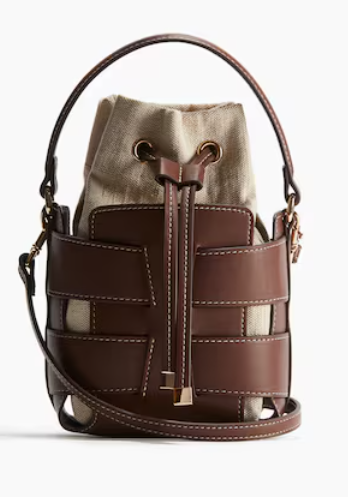
\includegraphics[width=3cm]{7176748c4afb4254a609e009d65c253a.png}};
\end{tikzpicture}


\cvsection{SUMMARY}
Passionné par l’informatique et le marketing digital, j’ai consolidé mes compétences en configuration de postes, maintenance de réseaux et support utilisateur. Mon année d’alternance à la DSI de la Mairie du Gosier m’a permis de gérer des projets numériques et de contribuer à la stratégie de communication en ligne. Rigoureux et orienté résultats, je souhaite désormais mettre mon expertise au service de votre organisation à temps plein. Mon objectif est de garantir la performance de vos systèmes tout en valorisant votre présence digitale.

\cvsection{SKILLS}
\begin{itemize}[leftmargin=*]
\item Marketing
\item Digital
\item Réseaux
\item Maintenance
\item Assistance
\item Support
\item Configuration\end{itemize}

\cvsection{LANGUAGES}
\begin{itemize}[leftmargin=*]
\item English - \textcolor{gray}{}
\item Espagnol - \textcolor{gray}{}\end{itemize}

\cvsection{INTERESTS}
\begin{itemize}[leftmargin=*]
\item Lectur
\item Sports
\item Musique
\item Voyage
\end{itemize}

\end{paracol}
\end{document}
